\begin{figure}[h!]
	\centering
	
	
	
	\tikzset{every picture/.style={line width=0.75pt}} %set default line width to 0.75pt        
	
	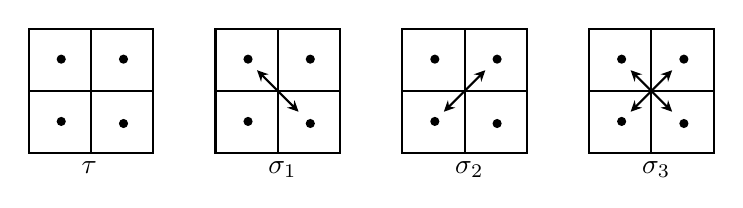
\begin{tikzpicture}[x=0.75pt,y=0.75pt,yscale=-1,xscale=1]
		%uncomment if require: \path (0,300); %set diagram left start at 0, and has height of 300
		
		%Shape: Square [id:dp32281460324226097] 
		\draw   (140,110) -- (200,110) -- (200,170) -- (140,170) -- cycle ;
		%Shape: Square [id:dp8196638610158489] 
		\draw   (140,140) -- (170,140) -- (170,170) -- (140,170) -- cycle ;
		%Shape: Square [id:dp5774035572053016] 
		\draw   (170,110) -- (200,110) -- (200,140) -- (170,140) -- cycle ;
		%Shape: Circle [id:dp09891447874029646] 
		\draw  [fill={rgb, 255:red, 0; green, 0; blue, 0 }  ,fill opacity=1 ] (154,154.67) .. controls (154,153.75) and (154.75,153) .. (155.67,153) .. controls (156.59,153) and (157.33,153.75) .. (157.33,154.67) .. controls (157.33,155.59) and (156.59,156.33) .. (155.67,156.33) .. controls (154.75,156.33) and (154,155.59) .. (154,154.67) -- cycle ;
		%Shape: Circle [id:dp22116361037170384] 
		\draw  [fill={rgb, 255:red, 0; green, 0; blue, 0 }  ,fill opacity=1 ] (154,124.67) .. controls (154,123.75) and (154.75,123) .. (155.67,123) .. controls (156.59,123) and (157.33,123.75) .. (157.33,124.67) .. controls (157.33,125.59) and (156.59,126.33) .. (155.67,126.33) .. controls (154.75,126.33) and (154,125.59) .. (154,124.67) -- cycle ;
		%Shape: Circle [id:dp9650296343672273] 
		\draw  [fill={rgb, 255:red, 0; green, 0; blue, 0 }  ,fill opacity=1 ] (184,124.67) .. controls (184,123.75) and (184.75,123) .. (185.67,123) .. controls (186.59,123) and (187.33,123.75) .. (187.33,124.67) .. controls (187.33,125.59) and (186.59,126.33) .. (185.67,126.33) .. controls (184.75,126.33) and (184,125.59) .. (184,124.67) -- cycle ;
		%Shape: Circle [id:dp04305617583331389] 
		\draw  [fill={rgb, 255:red, 0; green, 0; blue, 0 }  ,fill opacity=1 ] (184,155.67) .. controls (184,154.75) and (184.75,154) .. (185.67,154) .. controls (186.59,154) and (187.33,154.75) .. (187.33,155.67) .. controls (187.33,156.59) and (186.59,157.33) .. (185.67,157.33) .. controls (184.75,157.33) and (184,156.59) .. (184,155.67) -- cycle ;
		%Shape: Square [id:dp9546517027938655] 
		\draw   (230,110) -- (290,110) -- (290,170) -- (230,170) -- cycle ;
		%Shape: Square [id:dp9796040587153678] 
		\draw   (230,140) -- (260,140) -- (260,170) -- (230,170) -- cycle ;
		%Shape: Square [id:dp44002801088017396] 
		\draw   (260,110) -- (290,110) -- (290,140) -- (260,140) -- cycle ;
		%Shape: Circle [id:dp8334842171707744] 
		\draw  [fill={rgb, 255:red, 0; green, 0; blue, 0 }  ,fill opacity=1 ] (244,154.67) .. controls (244,153.75) and (244.75,153) .. (245.67,153) .. controls (246.59,153) and (247.33,153.75) .. (247.33,154.67) .. controls (247.33,155.59) and (246.59,156.33) .. (245.67,156.33) .. controls (244.75,156.33) and (244,155.59) .. (244,154.67) -- cycle ;
		%Shape: Circle [id:dp7038719736923629] 
		\draw  [fill={rgb, 255:red, 0; green, 0; blue, 0 }  ,fill opacity=1 ] (244,124.67) .. controls (244,123.75) and (244.75,123) .. (245.67,123) .. controls (246.59,123) and (247.33,123.75) .. (247.33,124.67) .. controls (247.33,125.59) and (246.59,126.33) .. (245.67,126.33) .. controls (244.75,126.33) and (244,125.59) .. (244,124.67) -- cycle ;
		%Shape: Circle [id:dp31839873684913567] 
		\draw  [fill={rgb, 255:red, 0; green, 0; blue, 0 }  ,fill opacity=1 ] (274,124.67) .. controls (274,123.75) and (274.75,123) .. (275.67,123) .. controls (276.59,123) and (277.33,123.75) .. (277.33,124.67) .. controls (277.33,125.59) and (276.59,126.33) .. (275.67,126.33) .. controls (274.75,126.33) and (274,125.59) .. (274,124.67) -- cycle ;
		%Shape: Circle [id:dp4037814749975406] 
		\draw  [fill={rgb, 255:red, 0; green, 0; blue, 0 }  ,fill opacity=1 ] (274,155.67) .. controls (274,154.75) and (274.75,154) .. (275.67,154) .. controls (276.59,154) and (277.33,154.75) .. (277.33,155.67) .. controls (277.33,156.59) and (276.59,157.33) .. (275.67,157.33) .. controls (274.75,157.33) and (274,156.59) .. (274,155.67) -- cycle ;
		%Shape: Square [id:dp21356453024304045] 
		\draw   (320,110) -- (380,110) -- (380,170) -- (320,170) -- cycle ;
		%Shape: Square [id:dp8300128863871687] 
		\draw   (320,140) -- (350,140) -- (350,170) -- (320,170) -- cycle ;
		%Shape: Square [id:dp3841760757181829] 
		\draw   (350,110) -- (380,110) -- (380,140) -- (350,140) -- cycle ;
		%Shape: Circle [id:dp06400640599899687] 
		\draw  [fill={rgb, 255:red, 0; green, 0; blue, 0 }  ,fill opacity=1 ] (334,154.67) .. controls (334,153.75) and (334.75,153) .. (335.67,153) .. controls (336.59,153) and (337.33,153.75) .. (337.33,154.67) .. controls (337.33,155.59) and (336.59,156.33) .. (335.67,156.33) .. controls (334.75,156.33) and (334,155.59) .. (334,154.67) -- cycle ;
		%Shape: Circle [id:dp4219802758838924] 
		\draw  [fill={rgb, 255:red, 0; green, 0; blue, 0 }  ,fill opacity=1 ] (334,124.67) .. controls (334,123.75) and (334.75,123) .. (335.67,123) .. controls (336.59,123) and (337.33,123.75) .. (337.33,124.67) .. controls (337.33,125.59) and (336.59,126.33) .. (335.67,126.33) .. controls (334.75,126.33) and (334,125.59) .. (334,124.67) -- cycle ;
		%Shape: Circle [id:dp12957899145925378] 
		\draw  [fill={rgb, 255:red, 0; green, 0; blue, 0 }  ,fill opacity=1 ] (364,124.67) .. controls (364,123.75) and (364.75,123) .. (365.67,123) .. controls (366.59,123) and (367.33,123.75) .. (367.33,124.67) .. controls (367.33,125.59) and (366.59,126.33) .. (365.67,126.33) .. controls (364.75,126.33) and (364,125.59) .. (364,124.67) -- cycle ;
		%Shape: Circle [id:dp09206954889493102] 
		\draw  [fill={rgb, 255:red, 0; green, 0; blue, 0 }  ,fill opacity=1 ] (364,155.67) .. controls (364,154.75) and (364.75,154) .. (365.67,154) .. controls (366.59,154) and (367.33,154.75) .. (367.33,155.67) .. controls (367.33,156.59) and (366.59,157.33) .. (365.67,157.33) .. controls (364.75,157.33) and (364,156.59) .. (364,155.67) -- cycle ;
		%Shape: Square [id:dp38707064557107107] 
		\draw   (410,110) -- (470,110) -- (470,170) -- (410,170) -- cycle ;
		%Shape: Square [id:dp016467202872691322] 
		\draw   (410,140) -- (440,140) -- (440,170) -- (410,170) -- cycle ;
		%Shape: Square [id:dp24812893227031285] 
		\draw   (440,110) -- (470,110) -- (470,140) -- (440,140) -- cycle ;
		%Shape: Circle [id:dp18320251504349438] 
		\draw  [fill={rgb, 255:red, 0; green, 0; blue, 0 }  ,fill opacity=1 ] (424,154.67) .. controls (424,153.75) and (424.75,153) .. (425.67,153) .. controls (426.59,153) and (427.33,153.75) .. (427.33,154.67) .. controls (427.33,155.59) and (426.59,156.33) .. (425.67,156.33) .. controls (424.75,156.33) and (424,155.59) .. (424,154.67) -- cycle ;
		%Shape: Circle [id:dp1417318830130958] 
		\draw  [fill={rgb, 255:red, 0; green, 0; blue, 0 }  ,fill opacity=1 ] (424,124.67) .. controls (424,123.75) and (424.75,123) .. (425.67,123) .. controls (426.59,123) and (427.33,123.75) .. (427.33,124.67) .. controls (427.33,125.59) and (426.59,126.33) .. (425.67,126.33) .. controls (424.75,126.33) and (424,125.59) .. (424,124.67) -- cycle ;
		%Shape: Circle [id:dp5953928915650424] 
		\draw  [fill={rgb, 255:red, 0; green, 0; blue, 0 }  ,fill opacity=1 ] (454,124.67) .. controls (454,123.75) and (454.75,123) .. (455.67,123) .. controls (456.59,123) and (457.33,123.75) .. (457.33,124.67) .. controls (457.33,125.59) and (456.59,126.33) .. (455.67,126.33) .. controls (454.75,126.33) and (454,125.59) .. (454,124.67) -- cycle ;
		%Shape: Circle [id:dp5197879342370941] 
		\draw  [fill={rgb, 255:red, 0; green, 0; blue, 0 }  ,fill opacity=1 ] (454,155.67) .. controls (454,154.75) and (454.75,154) .. (455.67,154) .. controls (456.59,154) and (457.33,154.75) .. (457.33,155.67) .. controls (457.33,156.59) and (456.59,157.33) .. (455.67,157.33) .. controls (454.75,157.33) and (454,156.59) .. (454,155.67) -- cycle ;
		%Straight Lines [id:da1668296738798587] 
		\draw    (252.12,132.12) -- (267.88,147.88) ;
		\draw [shift={(270,150)}, rotate = 225] [fill={rgb, 255:red, 0; green, 0; blue, 0 }  ][line width=0.08]  [draw opacity=0] (5.36,-2.57) -- (0,0) -- (5.36,2.57) -- (3.56,0) -- cycle    ;
		\draw [shift={(250,130)}, rotate = 45] [fill={rgb, 255:red, 0; green, 0; blue, 0 }  ][line width=0.08]  [draw opacity=0] (5.36,-2.57) -- (0,0) -- (5.36,2.57) -- (3.56,0) -- cycle    ;
		%Straight Lines [id:da6153426025313546] 
		\draw    (357.88,132.12) -- (342.12,147.88) ;
		\draw [shift={(340,150)}, rotate = 315] [fill={rgb, 255:red, 0; green, 0; blue, 0 }  ][line width=0.08]  [draw opacity=0] (5.36,-2.57) -- (0,0) -- (5.36,2.57) -- (3.56,0) -- cycle    ;
		\draw [shift={(360,130)}, rotate = 135] [fill={rgb, 255:red, 0; green, 0; blue, 0 }  ][line width=0.08]  [draw opacity=0] (5.36,-2.57) -- (0,0) -- (5.36,2.57) -- (3.56,0) -- cycle    ;
		%Straight Lines [id:da47301045731826874] 
		\draw    (447.88,132.12) -- (432.12,147.88) ;
		\draw [shift={(430,150)}, rotate = 315] [fill={rgb, 255:red, 0; green, 0; blue, 0 }  ][line width=0.08]  [draw opacity=0] (5.36,-2.57) -- (0,0) -- (5.36,2.57) -- (3.56,0) -- cycle    ;
		\draw [shift={(450,130)}, rotate = 135] [fill={rgb, 255:red, 0; green, 0; blue, 0 }  ][line width=0.08]  [draw opacity=0] (5.36,-2.57) -- (0,0) -- (5.36,2.57) -- (3.56,0) -- cycle    ;
		%Straight Lines [id:da5852456111119229] 
		\draw    (432.12,132.12) -- (447.88,147.88) ;
		\draw [shift={(450,150)}, rotate = 225] [fill={rgb, 255:red, 0; green, 0; blue, 0 }  ][line width=0.08]  [draw opacity=0] (5.36,-2.57) -- (0,0) -- (5.36,2.57) -- (3.56,0) -- cycle    ;
		\draw [shift={(430,130)}, rotate = 45] [fill={rgb, 255:red, 0; green, 0; blue, 0 }  ][line width=0.08]  [draw opacity=0] (5.36,-2.57) -- (0,0) -- (5.36,2.57) -- (3.56,0) -- cycle    ;
		
		% Text Node
		\draw (164,172.4) node [anchor=north west][inner sep=0.75pt]    {$\tau $};
		% Text Node
		\draw (254,172.4) node [anchor=north west][inner sep=0.75pt]    {$\sigma _{1}$};
		% Text Node
		\draw (344,172.4) node [anchor=north west][inner sep=0.75pt]    {$\sigma _{2}$};
		% Text Node
		\draw (434,172.4) node [anchor=north west][inner sep=0.75pt]    {$\sigma _{3}$};
		
		
	\end{tikzpicture}
\end{figure}